%*****************************************
\chapter{Methods}\label{ch:Methods}
%*****************************************
\section{Shared Imbalance Detection (SID) tool}
The \ac{SID} tool consists of two components, a database and a python script. The database holds information about the array design, values used during the analysis and tables which are filled during analysis. The python script parses feature extraction files, importing information to the database and performing the Z score analysis with a combination of SQL commands and python functions.

\section{Requirements gathering}\label{Requirements}
To ensure the tool is fit for purpose requirements were agreed with key stakeholders in the Array and Bioinformatics teams within the Viapath Genetic Laboratories:
\subsection{Functional requirements}
\begin{itemize}
\item Use the signal intensities from the feature extraction file to identify \ac{CNV} independently of the hybridisation partner
\item An region of \ac{CNV} is defined as a minimum of three consecutive abnormal probes which is ended by three consecutive normal probes.
\item Report any common or overlapping regions of abnormal copy number present in both hybridisation partners.
\item The test is a screen, sensitivity favoured over specificity.
\end{itemize}
\subsection{Non functional requirements}
\begin{itemize}
\item In line with the existing departmental resources, experience and skill sets data will be stored in an MS-SQL database hosted by a remote server, ensuring long term support.
\item Any scripting should be performed in Python, in line with the existing department skill set to ensure long term support and development and code reviewed as per best practice guidelines. 
\item Python code must conform with the departmental Python style guide.
\item Code must be version controlled using Git.
\item Processing should be timely and able to be performed on existing desktop computers.
\item The feature extraction files are required for analysis by Genetic Scientists so must not be modified or moved from the current location.
\item Compatible with the trust operating system (Windows XP, with an upgrade to Windows 10 planned before 2018).
\item Able to be run from multiple computers within the department by multiple users.
\item Analysis must be reproducible.
\item The database must be in third normalised form to ensure data integrity.
\item \ac{SOP} and validation documentation in line with ISO accreditation requirements.
\item Validated in line with departmental and ISO quality procedures.
\end{itemize}
\subsection{Project management}
\begin{itemize}
\item Use an Agile development methodology to regularly test and refine the project (Figure \ref{fig:Agile}).
\begin{figure}[h]
\centering
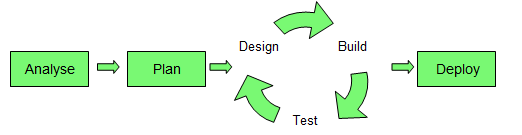
\includegraphics[width=1\linewidth]{./Figures/Agile}
\caption[Agile development methodology]{The agile software design methodology promotes regular testing to ensure the design is fit for purpose}
\label{fig:Agile}
\end{figure}
\item Use smartsheet (\url{https://www.smartsheet.com}) to set goals and monitor progress with stakeholders 
\item An electronic lab book is to be kept within the departmental wiki
\item Weekly meetings will be held with key stakeholders.
\end{itemize}

\section{Database infrastructure}
\subsection{SQL server}
Access to the MS-SQL hosted on the department server was not available during development. Installation of an MS-SQL server on the development system was also not possible at the start of the project so development was performed using a MySQL server (v5.6)\cite{mysql_mysql_????} running locally on a development PC running Windows 10. 

\subsection{Migration from development server (MYSQL) to production server (MS-SQL)}
The database was later transferred to a MS-SQL server (SQLExpress 2014 \cite{_sql_????}) on the development system using Microsoft SQL Server Migration Assistant (v5.3) for MySQL \cite{_microsoft_????}
\paragraph*{}
The MySQLdb python connector was replaced by PyODBC MSSQL connector \cite{pyodbc_mkleehammer/pyodbc_????} and tested to ensure no loss of function.

\subsection{HeidiSQL client}
Database development was performed using the HeidiSQL client (v9.1)\cite{heidisql_heidisql_2016}.

\section{SID - database design}
To minimise processing time only essential fields from the feature extraction file is imported to the database. The database is designed in third normalised form, storing numeric keys to prevent anomalies and to maximise the performance of joins. Array wide values are stored a single time in the feparam table, not for each feature.
\begin{figure}
\centering
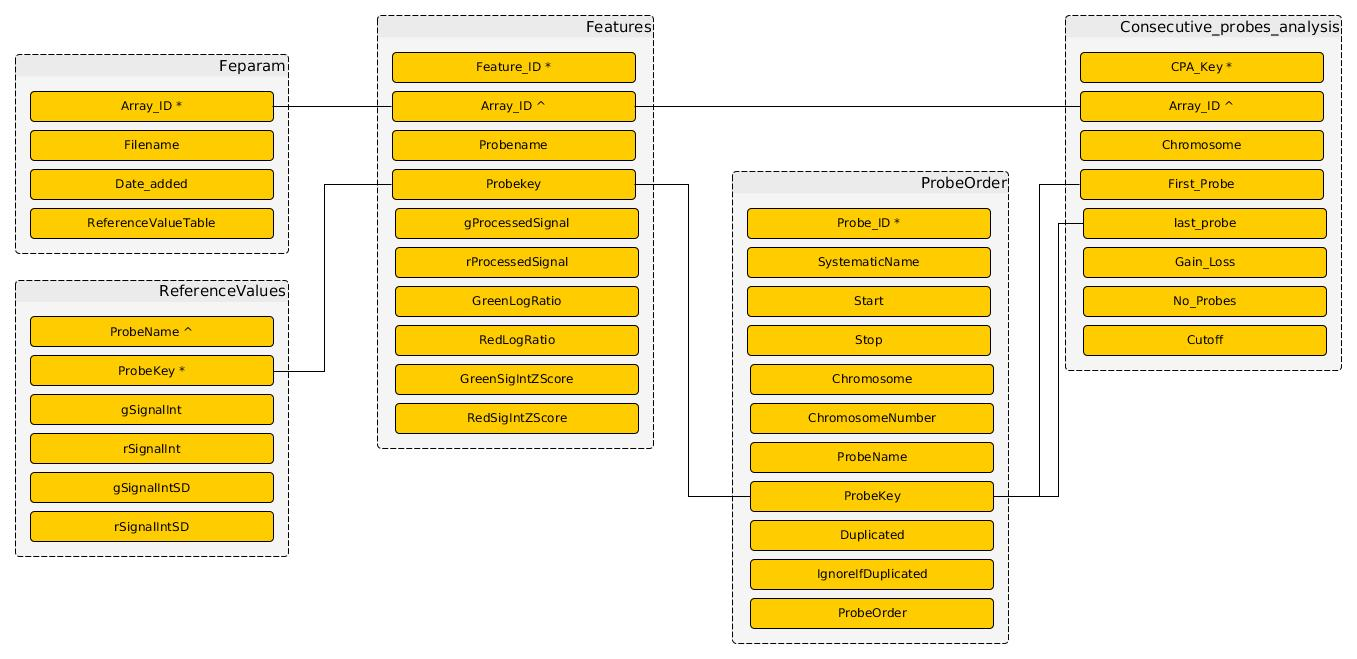
\includegraphics[width=1.2\linewidth]{./Figures/SIDdbschema-simple}
\caption[The SID database schema]{The SID database schema. Five tables are required.\string^ denotes an indexed field, * denotes a primary key. Lines denote how tables are joined.}
\label{fig:SIDdbschema-simple}
\end{figure}

\paragraph*{}
Five tables are required (Figure \ref{fig:SIDdbschema-simple}).The Feparam table holds the filename of the feature extraction file. Upon insertion an auto incrementing number is created as the primary key and used as the unique identifier for that array (Array\_ID). The Feparam table also records the reference table used and an automatic time stamp. 
\paragraph*{}
The array design is stored in the Probeorder table. Each probe has a numerical key (probekey) and it's order in genomic position (probeorder). Only non-control probes are stored and replicated probes flagged.
\paragraph*{}
The ReferenceValues table holds the average signal intensity and the standard deviation from the normal control population for each dye at each probe (see \ref{ch:createreference}).
\paragraph*{}
The Features table holds the analysis for each probe. Of the 42 fields only the probename and processed signals are imported. Remaining fields are populated during the analysis.
\paragraph*{}
Results of analysis are entered into the consecutive\_probe\_analysis table enabling the aberration to be fully characterised.

\subsection{Indexes and keys}
Each table has a primary key which is unique and indexed. 
Any columns which are joined to the primary key of another table are foreign keys.
Any columns used to join table are also indexed to improve performance.

\section{Importing and processing feature extraction files}
\subsection{Python}
Feature extraction files were parsed using Python (v2.7)\cite{python_software_foundation_python_2010}. The Anaconda Python distribution (v2.3.0) \cite{continuum_why_2016} was selected to make use of the pre-installed packages such as NumPy, SciPy and math packages. The package manager Conda was used to install the MySQLdb package (mysql-python v1.2.5)\cite{dustman2014} to access the MySQL database from python. 
\paragraph*{}
The Eclipse \ac{IDE} (Luna v 4.4.1) \cite{the_eclipse_foundation_eclipse_????} was used with the PyDev package (v 3.9.0) \cite{pydev_python_????} to develop and run Python scripts.
\paragraph*{}
The Pylint Python package (v 1.4.2) \cite{pylint_code_????} and autopep8 were used within Eclipse to apply the local Python style guide to the code.

\subsection{Version control}
Python code was version controlled using Git and backed up using GitHub (\url{https://github.com/aledj2/FeatureExtraction}).


\section{SID - pprocessing feature extraction files}
An overview of the SID python script can be seen in Figure \ref{fig:program_overview_extensive2} .

\begin{figure}
\centering
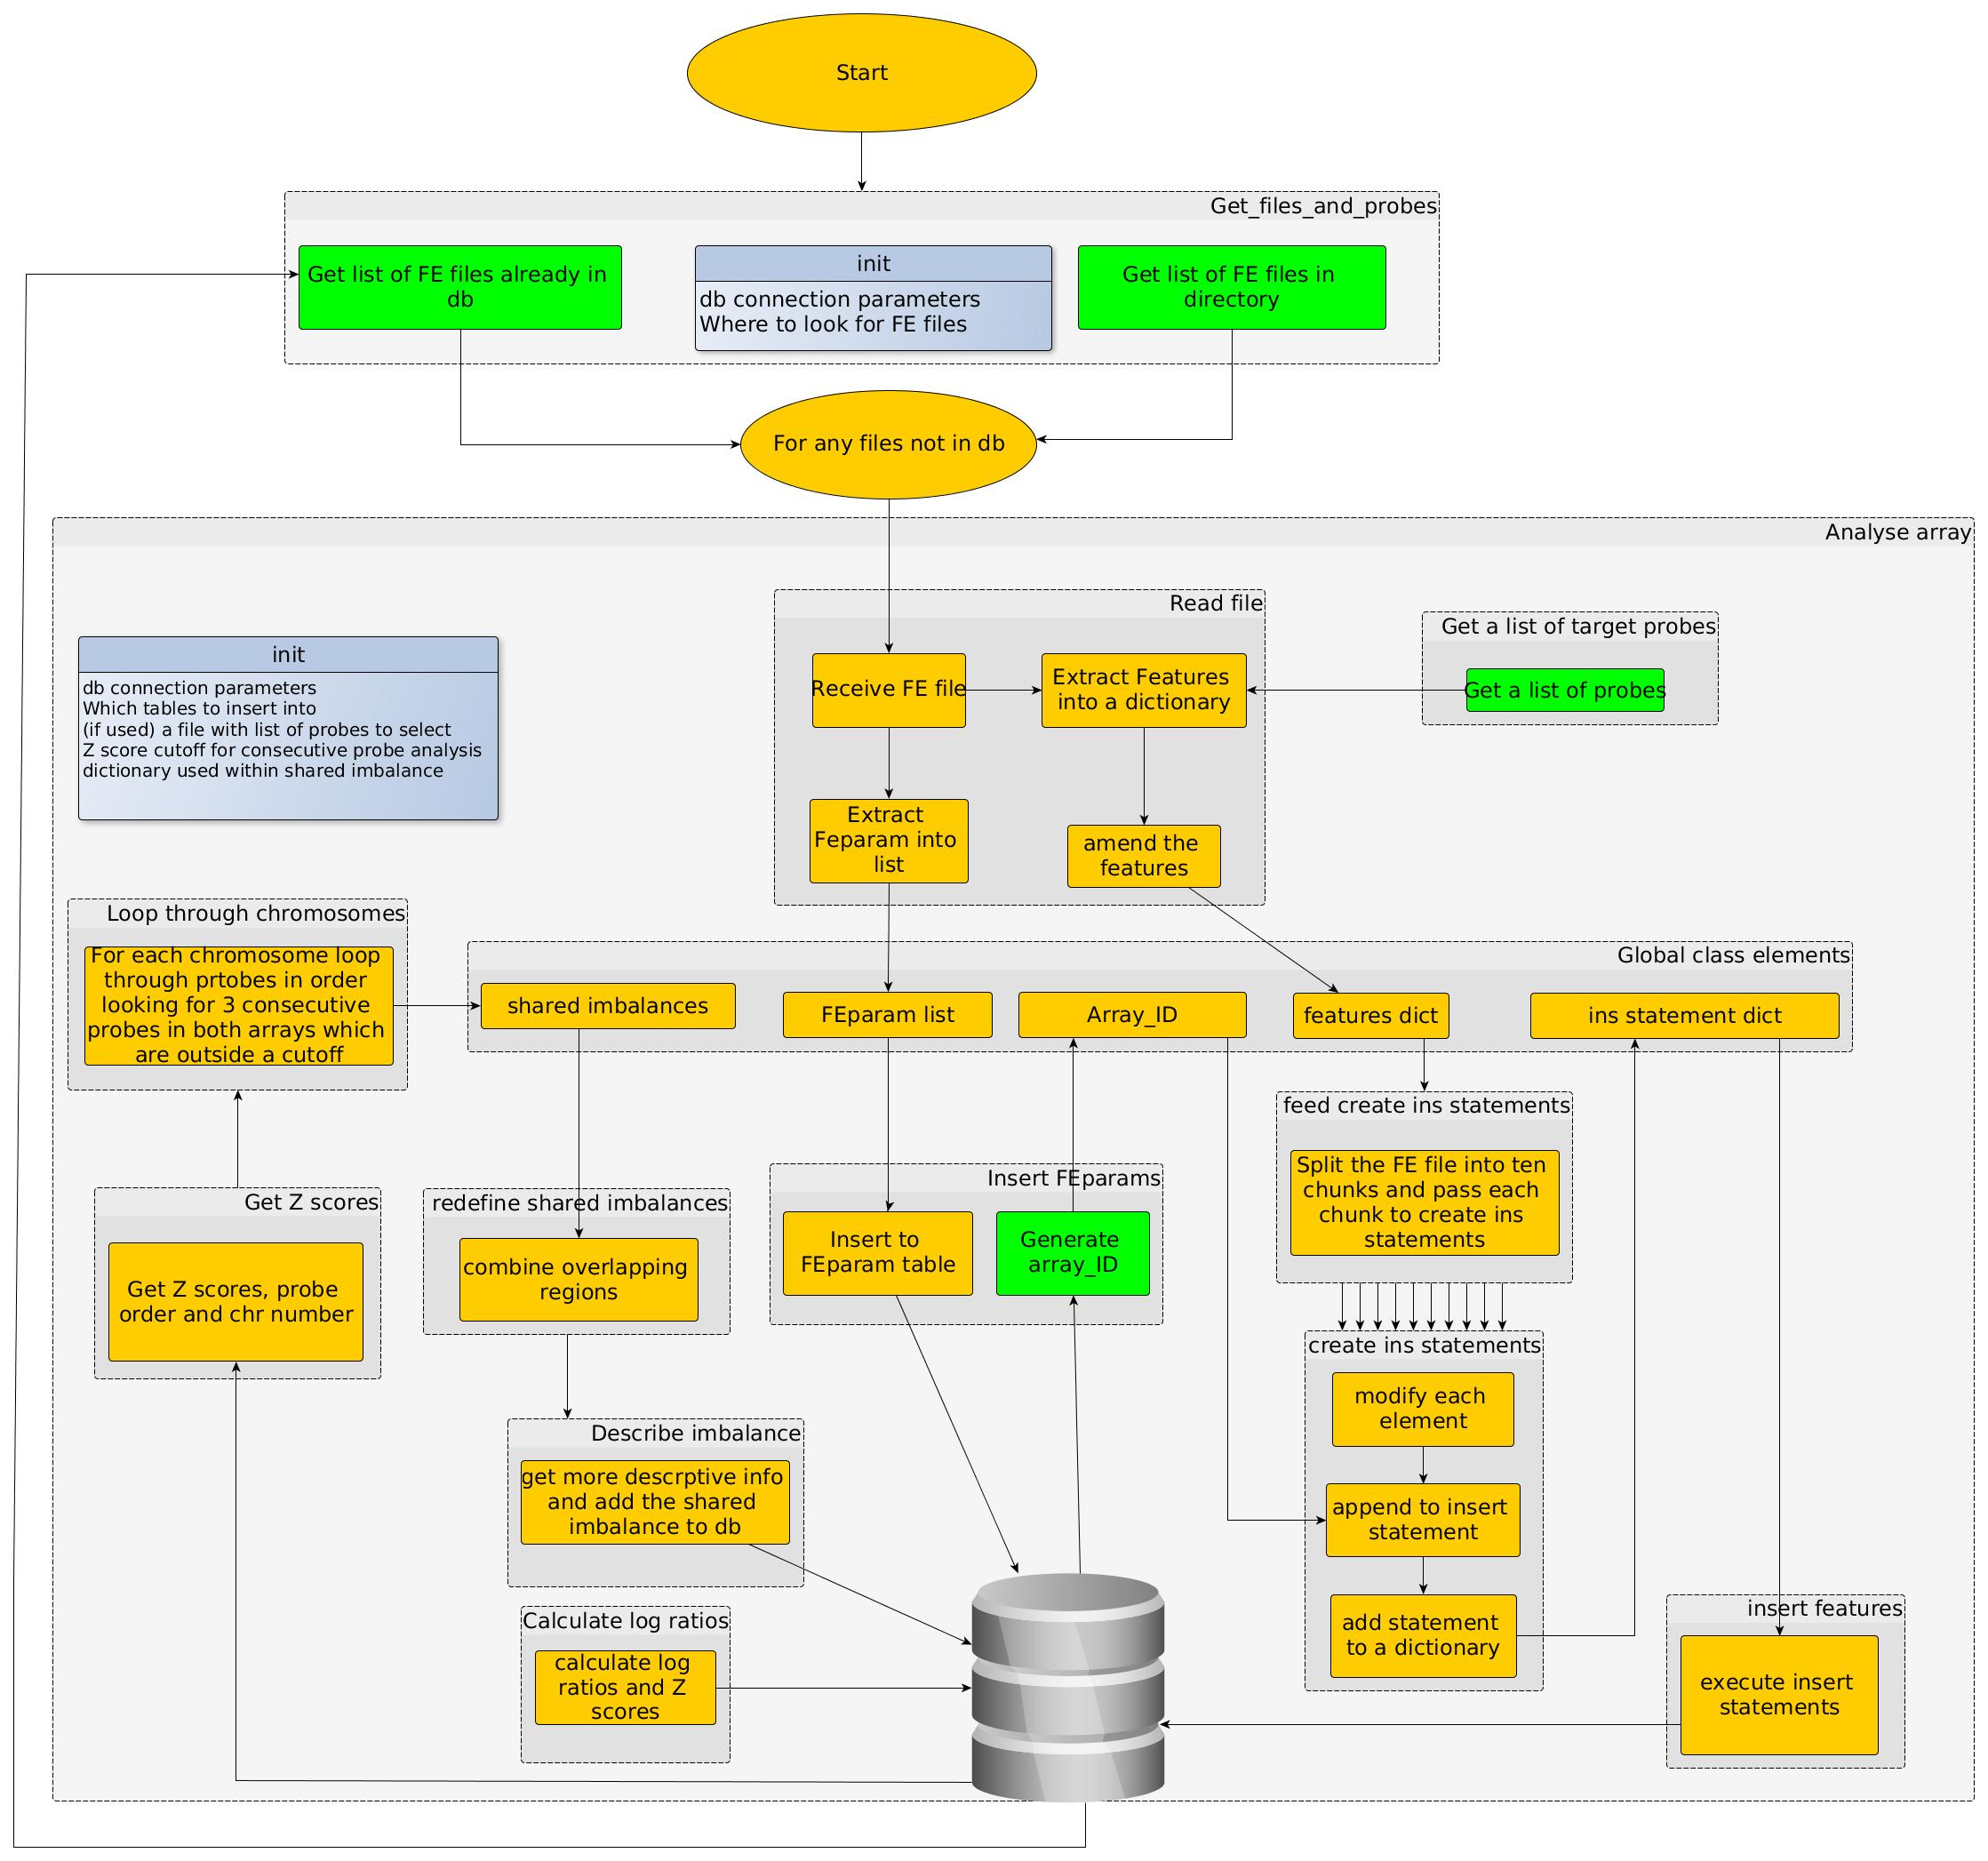
\includegraphics[width=1.2\linewidth]{./Figures/program_overview_extensive2}
\caption[A visual representation of the SID python script]{A visual representation of the SID python script. The Get\_files\_and\_probes class compares the list of feature extraction files within a directory to the feparam table.\\ Each array yet to be analysed is passed to Analyse\_array class. The read file module extracts the relevant information into dictionaries. The insert FEparams module enters the filename to the database and captures the primary key assigned (the array\_ID). The features section of the feature extraction file is broken into 10 and inserted with the array\_ID.\\ The calculate log ratios module applies an update statement to calculate Z scores and log ratios. The get Z scores module takes these Z scores and identifies shared trios of abnormal probes, combining overlapping or neighbouring calls and storing results. Functions coloured green read from the database, yellow process data and blue are \_\_init\_\_ modules which initialise variables for the class}
\label{fig:program_overview_extensive2}
\end{figure}

\section{Detection of CNV}
\subsection{Choice of algorithm (Z score)}
A Z score analysis method was selected for the analysis as the characterisation of breakpoints is not as critical as in routine analysis and this algorithm is simple to implement, maintain and troubleshoot, without the need for any additional software such as R.
\paragraph*{}
A Z score (equation \ref{eq:Zscore}) provides a measure of how many standard deviations the signal intensity of a probe is from the mean of a normal population. A threshold can then be applied to score probes as normal or abnormal.
\begin{equation} \label{eq:Zscore}
Z = \frac{Signal\ Intensity - Mean}{SD}
\end{equation}

\subsection{Creating a normal reference range} \label{ch:createreference}
100 arrays with no reported CNV were selected to create a reference range. Care was taken not to select only high quality arrays as this may result in many false positive calls in poor quality arrays.
\paragraph*{}
The 100 arrays were imported into the database. A Python script calculated the average signal intensity and standard deviation for each dye at each probe.
These values are held in the ReferenceValues table which is versioned using the date as the reference may require periodically recalculating.
\paragraph*{}
The ReferenceValues table used is specified within the SID  Python script and recorded in the Feparams table, allowing analysis to be repeated after the reference range has been recalculated.
\subsubsection{Normal distribution of reference range}
Z scores require normally distributed reference ranges. However some probes will not be normally distributed for example if they are within a common CNV. 
\begin{figure}[h]
\centering
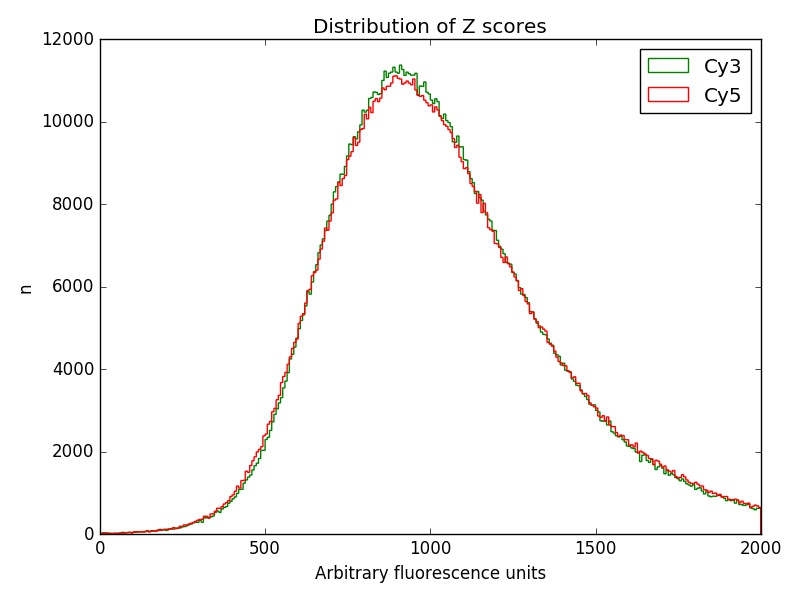
\includegraphics[width=1\linewidth]{./Figures/distributionof30arrays}
\caption[The distribution of signal intensities from 30 arrays]{The distribution of signal intensities from all probes from 30 arrays is slightly positively skewed}
\label{fig:distributionof30arrays}
\end{figure}

\paragraph*{}
A histogram of the signal intensities of all probes from 30 arrays (Figure \ref{fig:distributionof30arrays}) shows a slightly positively skewed distribution. This it to be expected as the signal intensities cannot be negative and gains in copy number is seen more commonly than losses \cite{zhang2009}.

\subsection{Determining if a probe is normal or abnormal}
The Z score for each dye at each probe is calculated during the import of data and stored within the Features table. 
The Z score is a measure of how many standard deviations from the mean the signal intensity of the probe is. A threshold is required to define a probe as abnormal.
\begin{figure}
\centering
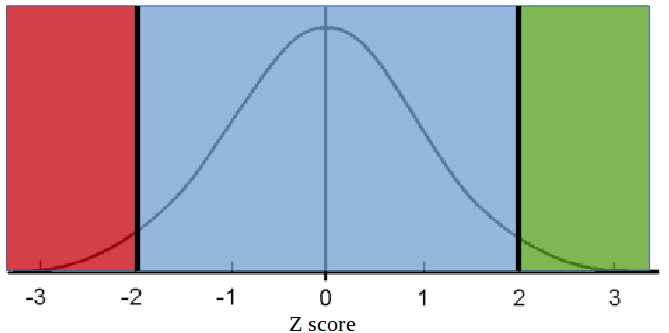
\includegraphics[width=1\linewidth]{./Figures/normaldist}
\caption[The normal distribution]{Thresholds define probes as abnormal or normal. A more extreme threshold will define fewer probes as abnormal.}
\label{fig:normaldist}
\end{figure}

\paragraph*{}
Z scores are two tailed so probes with a Z score above the threshold are defined as gains and Z scores below the negative threshold are defined as loss (Figure \ref{fig:normaldist}).

\subsection{Duplicated probes}
For the 29 duplicated probes an average of the signal intensities is taken.
\subsection{Determining if a region is normal or abnormal}
To combine abnormal probes into segments a slightly different approach was taken to the Z score algorithm described by Agilent \cite{agilent_technologies_agilent_2011}.

\begin{figure}
\centering
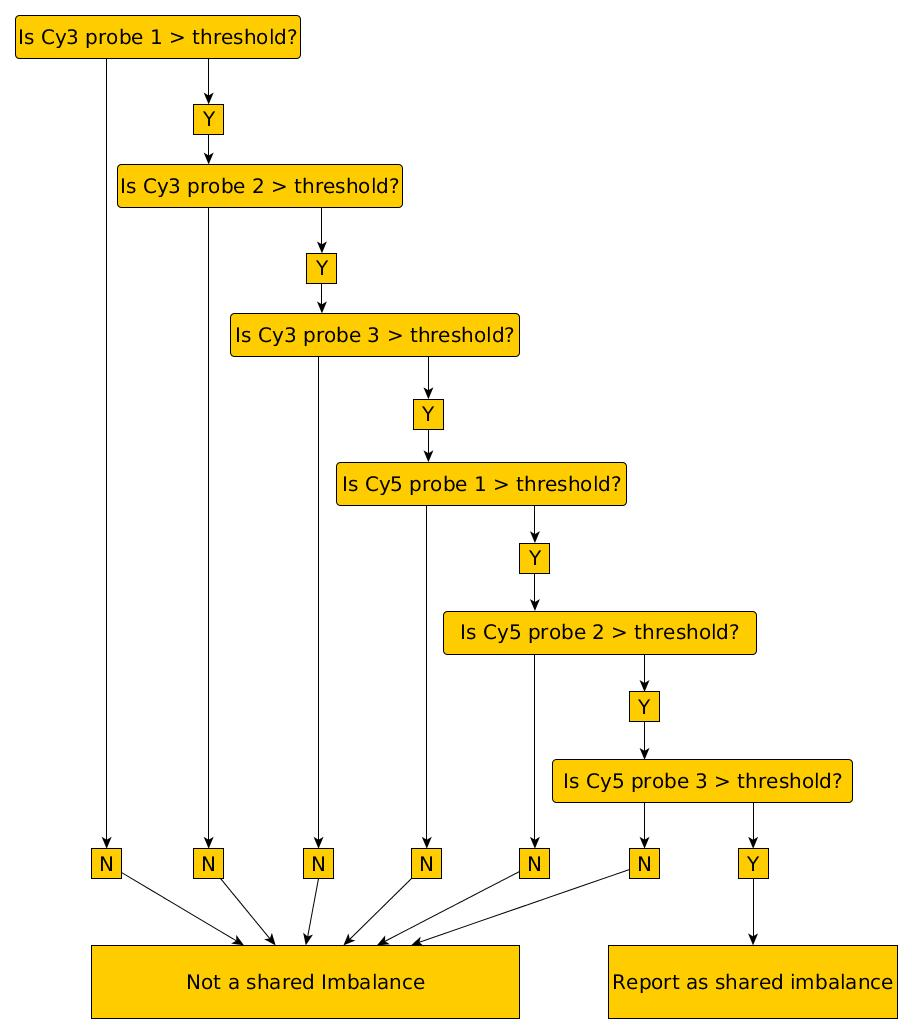
\includegraphics[width=0.7\linewidth]{./Figures/consecutiveprobeanalysis}
\caption[Consecutive probe analysis algorithm]{Consecutive probe analysis algorithm. To determine if the sliding window of three probes is abnormal in both samples the Z score of each probe is tested in succession. The threshold is defined in SID python script.\\
This process is repeated assessing if the Z score is less than the negative threshold.}
\label{fig:consecutiveprobeanalysis}
\end{figure}

\begin{figure}
\centering
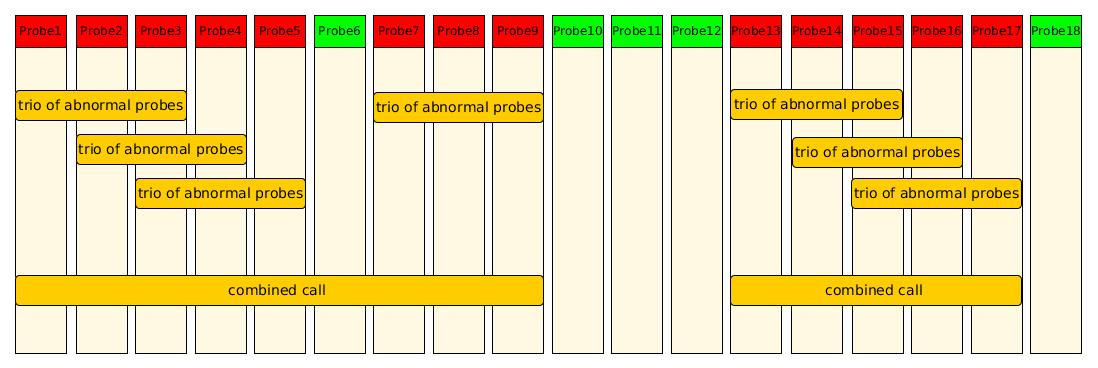
\includegraphics[width=1\linewidth]{./Figures/combiningtrioofprobes}
\caption[Trios of abnormal probes are combined into a single call ]{Trios of probes are combined into a single call in line with the analysis strategy. Abnormal probes are represented in red and normal probes represented in green. Trios of shared imbalances are shown. Overlapping and neighbouring calls are combined if they are separated by less than three normal probes (eg probes 10-12).}
\label{fig:combiningtrioofprobes}
\end{figure}

\paragraph*{}
Aberrations below three probes are not reported so a sliding window of three probes was used, identifying shared CNV of three consecutive probes (Figure \ref{fig:consecutiveprobeanalysis}). The window moved along the entire chromosome creating overlapping tiles (Figure \ref{fig:combiningtrioofprobes}).

\paragraph*{}
Trios of shared CNV are then combined in line with routine analysis, combining regions unless separated by 3 or more normal probes (Figure \ref{fig:combiningtrioofprobes}).
\section{Creation of true positive feature extraction files}
SID underwent three stages of development.
\subsection{Training cases}
A Python script was written to create true positive feature extraction files using feature extraction files with reported aberrations. 
\paragraph*{}
Probes within the reported region were identified and a new feature extraction file was created where the Cy5 signal intensity was replaced by the Cy3 signal intensity. This was repeated replacing the Cy3 signal intensity with the Cy5 signal intensity.
\paragraph*{}
The script created one true positive, with signal intensities representing an aberration in both hybridisation partners and one true negative file where both partners have normal signal intensities.
\paragraph*{}
This training set was used to investigate and define the parameters required to call a probe as abnormal. 
\subsection{Test cases}
The test set was used to ensure the parameters were not over-fitted to the training set. An updated strategy was applied to create the test set. Two samples which had exactly the same reported CNV were hybridised post-hoc. 
To ensure the signal intensities would be compared against the correct reference range a sample labelled with Cy3 was paired with one labelled with Cy5. 
\paragraph*{}
EvE, a Python script used for the post-hoc hybridisation of arrays in \ac{PGD} cases, parses two feature extraction files, extracting all measurements for both samples on both arrays, and creates a new feature extraction file where the Cy3 measurements are populated from the Cy3 sample from the first file and the Cy5 measurements from the Cy5 sample from the second file.

\paragraph*{}
The test cases were reported to have one of the most commonly reported CNV, representing a range of sizes and loss and gains (Table \ref{tab:testset_calls}).

\begin{table}
\caption{Cases with one of the 9 most common CNV were used to create the test set}
\label{tab:testset_calls}
\resizebox{\textwidth}{!}{%
\begin{tabular}{|c|c|c|c|}
\hline Aberration  & Copies & Number of Probes & Number of arrays \\ 
\hline 15:22765627-2308509 & 1 & 11 & 9 \\ 
\hline 16:29673953-30198600 & 1 & 34 & 9 \\ 
\hline 16:29673953-30198600 & 3 & 34 & 10 \\ 
\hline 22:18896971-211440514 & 1 & 750 & 8 \\ 
\hline 15:30933080-32514980 & 1 & 30 & 6 \\ 
\hline 16:21806298-22407931 & 1 & 15 & 10 \\ 
\hline 7:72700413-74142327 & 1 & 43 & 6 \\ 
\hline 1:145413387-145747269 & 3 & 21 & 5 \\ 
\hline 6:26440746-26463502 & 1 & 3 & 6 \\ 
\hline 
\end{tabular}%
}
\end{table}

\subsection{Prospective cases}
121 unmodified array files used to create the test set were used as a prospective trial to indicate the expected number of calls seen in routine analysis.

\section{Definition of true positive and false positive calls}
A true positive call is defined as any call overlapping with the reported CNV. There may be multiple calls within this region.
\paragraph*{}
A false positive call does not share a single probe with the reported CNV.

\subsection{Unknown true positive calls}
In the training and test sets the true positive calls are defined as those which have been reported as clinically significant based on the referral reason however on average an array will have 3-4 regions of CNV \cite{joowook_ahn_average_2015}. These calls can be false positive calls made by the algorithm or real benign calls in regions of common copy number variation.
\paragraph*{}
Therefore the number of false positive calls will be inflated and the true specificity unknown.